\documentclass[border=15pt]{standalone}
\usepackage{tikz}
\usetikzlibrary{positioning, shapes.geometric, arrows.meta, calc, fit, backgrounds}

% Colors
\definecolor{TokenColor}{RGB}{156,39,176}
\definecolor{TransColor}{RGB}{33,150,243}
\definecolor{ConcatColor}{RGB}{255,152,0}
\definecolor{HeadColor}{RGB}{233,30,99}
\definecolor{OutputColor}{RGB}{76,175,80}

\begin{document}
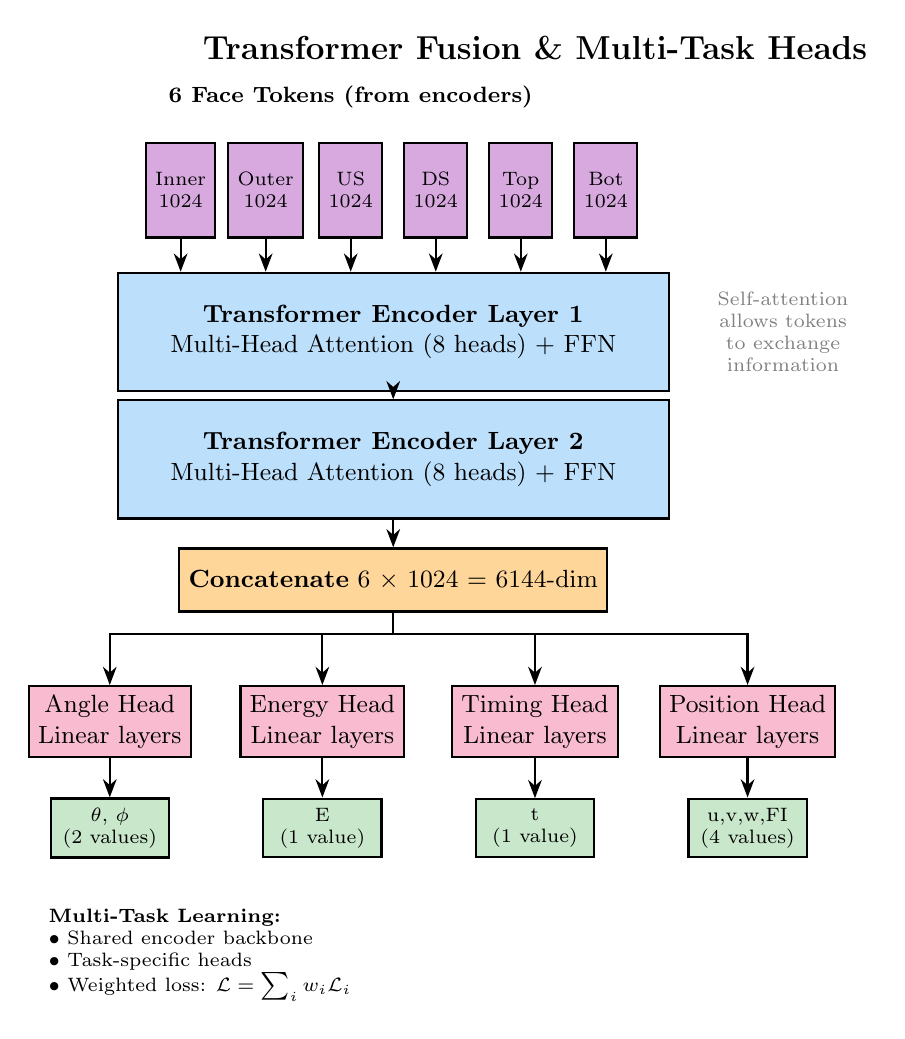
\begin{tikzpicture}[
    scale=0.9,
    every node/.style={font=\small},
    >=Stealth,
    token/.style={rectangle, draw, thick, fill=TokenColor!40, minimum width=0.8cm, minimum height=1.2cm, align=center, font=\scriptsize},
    transblock/.style={rectangle, draw, thick, fill=TransColor!30, minimum width=3cm, minimum height=1.2cm, align=center},
    concat/.style={rectangle, draw, thick, fill=ConcatColor!40, minimum width=5cm, minimum height=0.8cm, align=center},
    head/.style={rectangle, draw, thick, fill=HeadColor!30, minimum width=2cm, minimum height=0.8cm, align=center},
    output/.style={rectangle, draw, thick, fill=OutputColor!30, minimum width=1.5cm, minimum height=0.6cm, align=center, font=\scriptsize},
]

% Title
\node[font=\large\bfseries] at (5, 8) {Transformer Fusion \& Multi-Task Heads};

% 6 Face Tokens
\node[token] (t1) at (0, 6) {Inner\\1024};
\node[token] (t2) at (1.2, 6) {Outer\\1024};
\node[token] (t3) at (2.4, 6) {US\\1024};
\node[token] (t4) at (3.6, 6) {DS\\1024};
\node[token] (t5) at (4.8, 6) {Top\\1024};
\node[token] (t6) at (6.0, 6) {Bot\\1024};

\node[above=0.3cm of t3, font=\footnotesize\bfseries] {6 Face Tokens (from encoders)};

% Transformer Encoder
\node[transblock, minimum width=7cm, minimum height=1.5cm] (trans1) at (3, 4) {
    \textbf{Transformer Encoder Layer 1}\\
    Multi-Head Attention (8 heads) + FFN
};

\node[transblock, minimum width=7cm, minimum height=1.5cm] (trans2) at (3, 2.2) {
    \textbf{Transformer Encoder Layer 2}\\
    Multi-Head Attention (8 heads) + FFN
};

% Arrows to transformer
\foreach \t in {t1, t2, t3, t4, t5, t6} {
    \draw[->, thick] (\t.south) -- (\t.south |- trans1.north);
}

% Arrow between transformer layers
\draw[->, thick] (trans1.south) -- (trans2.north);

% Concatenate
\node[concat] (concat) at (3, 0.5) {\textbf{Concatenate} 6 $\times$ 1024 = 6144-dim};
\draw[->, thick] (trans2.south) -- (concat.north);

% Task Heads
\node[head] (angle_head) at (-1, -1.5) {Angle Head\\Linear layers};
\node[head] (energy_head) at (2, -1.5) {Energy Head\\Linear layers};
\node[head] (timing_head) at (5, -1.5) {Timing Head\\Linear layers};
\node[head] (pos_head) at (8, -1.5) {Position Head\\Linear layers};

% Arrows to heads
\draw[->, thick] (concat.south) -- ++(0, -0.3) -| (angle_head.north);
\draw[->, thick] (concat.south) -- ++(0, -0.3) -| (energy_head.north);
\draw[->, thick] (concat.south) -- ++(0, -0.3) -| (timing_head.north);
\draw[->, thick] (concat.south) -- ++(0, -0.3) -| (pos_head.north);

% Outputs
\node[output] (angle_out) at (-1, -3) {$\theta$, $\phi$\\(2 values)};
\node[output] (energy_out) at (2, -3) {E\\(1 value)};
\node[output] (timing_out) at (5, -3) {t\\(1 value)};
\node[output] (pos_out) at (8, -3) {u,v,w,FI\\(4 values)};

\draw[->, thick] (angle_head.south) -- (angle_out.north);
\draw[->, thick] (energy_head.south) -- (energy_out.north);
\draw[->, thick] (timing_head.south) -- (timing_out.north);
\draw[->, thick] (pos_head.south) -- (pos_out.north);

% Dimensions annotation
\node[font=\scriptsize, gray, align=center] at (8.5, 4) {Self-attention\\allows tokens\\to exchange\\information};

% Multi-task note
\node[font=\scriptsize, align=left, anchor=north west] at (-2, -4) {
    \textbf{Multi-Task Learning:}\\
    $\bullet$ Shared encoder backbone\\
    $\bullet$ Task-specific heads\\
    $\bullet$ Weighted loss: $\mathcal{L} = \sum_i w_i \mathcal{L}_i$
};

\end{tikzpicture}
\end{document}
